%%%% début de la page

\renewcommand{\thesubsection}{\textcolor{red}{\Roman{section}.\arabic{subsection}}}
\renewcommand{\thesubsubsection}{\textcolor{red}{\Roman{section}.\arabic{subsection}.\alph{subsubsection}}}

\setcounter{section}{0}
\setcounter{document}{0}
\sndEnTeteTPQuatre

\begin{center}
\begin{mdframed}[style=titr, leftmargin=60pt, rightmargin=60pt, innertopmargin=7pt, innerbottommargin=7pt, innerrightmargin=8pt, innerleftmargin=8pt]

\begin{center}
\large{\textbf{TP 4 : Comment bien choisir la verrerie pour mesurer des volumes précis ?}}
\end{center}


\end{mdframed}
\end{center}

%\begin{tableauCompetences}
 %   ANA & Mesurer des volumes & & & &
    
%\end{tableauCompetences}

%%%% objectifs
\begin{tcolorbox}[colback=blue!5!white,colframe=blue!75!black,title=Objectifs de la séance :]
\begin{itemize}
    \item Mesurer des masses pour étudier la variabilité du volume mesuré par une pièce de verrerie
  \item Choisir et utiliser la verrerie adaptée pour préparer une solution par dissolution
\end{itemize}
\end{tcolorbox}

%%%% contexte

\begin{tcolorbox}[colback=orange!5!white,colframe=orange!75!black,title= Scénario:]
Le laboratoire dispose de trois principales pièces de verrerie qu'on utilise couramment lors de manipulation complexe. Nommer ces trois verreries.
\begin{center}
    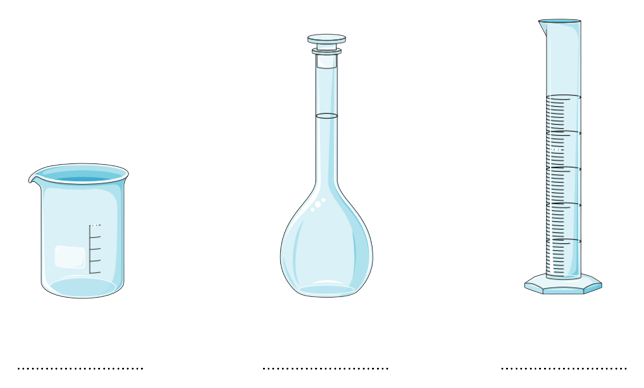
\includegraphics[scale=0.7]{Images/TP4/Verrerie_a_completer.png}
\end{center}
\problematique{On souhaite vérifier que la fiole jaugée est la pièce de verrerie la plus précise et la plus fidèle. Comment fait-on ?}
\end{tcolorbox}

\begin{tcolorbox}[colback=red!5!white,colframe=red!75!black,title= Consignes :]
\begin{itemize}
    \item Par binôme, nommer un responsable \og MES \fg : il aura la responsabilité de vérifier la bonne réalisation des mesures et de rentrer les valeurs expérimentales sur le fichier Excel du tableau. Nommer également un responsable \og COM \fg : il aura la responsabilité du compte-rendu et fera office de porte-parole du binôme,
    \item Faire attention à la verrerie lors de son utilisation,
    \item Respectez les consignes d'utilisation de la salle de chimie.
\end{itemize}

\end{tcolorbox}
\begin{mdframed}[style=autreexo]
\textbf{\bsc{Liste du matériel}}
\begin{itemize}
    \item une balance, 
    \item un bécher de 100~mL,
    \item une fiole jaugée de 25~mL,
    \item une éprouvette graduée de 50~mL,
    \item une pipette plastique,
    \item une pissette d'eau distillée,
    \item un ordinateur avec le tableur Excel.    
\end{itemize}
\end{mdframed}

\newpage
%%%% documents
\begin{doc}{Lecture d'un volume sur la verrerie}

\begin{wrapfigure}{r}{0.3\textwidth}
\vspace{-2cm}
    \centering
      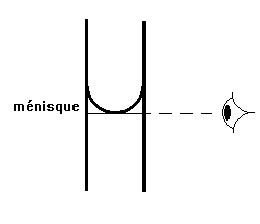
\includegraphics[width=0.27\textwidth]{Images/Activite/Chap1/Lecture_Verrerie.png}
  \end{wrapfigure}
  Lorsqu'on verse un liquide dans une pièce de verrerie (éprouvette, tube à essai, etc), il se forme un ménisque qui va perturber la lecture du volume sur la verrerie. Pour lire le volume occupé par un liquide, il faut positionner son \oe il sur le bas du ménisque.
\end{doc}

%%%%
\begin{doc}{Concentration en soluté}
  \label{doc:concentration}
  \vspace*{-24pt}
  \begin{tcolorbox}[colback=green!5!white,colframe=green!75!black,title=\textbf{Concentration massique}]
    La \important{concentration massique}, notée $c$, mesure la quantité de soluté présent dans une solution.
    C'est le rapport de la masse $m$ de \textbf{soluté} dissous dans le volume $V$ de la \textbf{solution}
    \begin{equation*}
      c = \frac{m_\text{soluté}}{V_\text{solution}}
    \end{equation*}
  \end{tcolorbox}
  
  \importantbox{Ne pas confondre \textbf{concentration massique} et \textbf{masse volumique} !
  La concentration mesure la masse de soluté contenue dans une solution.
  La masse volumique mesure la masse d'un échantillon contenue dans un volume donné.}
\end{doc}


%%%%
\newpage
\begin{doc}{Dakin}
  \label{doc:dakin}
  Le Dakin est une solution aqueuse d'hypochlorite de sodium \chemfig{Na ClO}.
  Du permanganate de potassium \chemfig{K MnO_4} est ajouté à la solution, pour qu'elle ne soit pas dégradée par l'exposition au rayonnement UV du Soleil.
  
  \fleche Le constructeur indique que la concentration de \chemfig{KMnO_4} est de l'ordre de $0,\!01 \unit{g/L}$ dans le Dakin.
\end{doc}


%%%%
\begin{doc}{Mesure de concentration}
  \label{doc:dosage}
  \vspace*{-24pt}
  \begin{definition}{Dosage}
    On parle de \important{dosage} quand on mesure la concentration d'une espèce chimique présente dans une solution.
    
    Un \important{dosage par étalonnage} consiste à déterminer la concentration d’une espèce chimique en comparant une grandeur physique caractéristique de la solution, à la même grandeur physique mesurée pour des solutions étalon.
  \end{definition}
  
 Une \textcolor{red}{\textbf{échelle de teinte} }permet de mesurer la concentration d'un soluté coloré. En effet, la teinte d'une solution est proportionnelle à la concentration en soluté.
  En préparant une série de solutions de concentrations connues, une \textbf{gamme}, et en comparant les teintes, on va pouvoir encadrer la valeur de la concentration de la solution que l'on veut mesurer.
  
  \bigskip
  
  \importantbox{Il faut comparer les teintes avec des verreries identiques, la teinte s'assombrit avec l'épaisseur. \newline
  La solution dont on veut mesurer la concentration doit avoir une teinte comprises dans la gamme réalisée !
  }
\end{doc}
 

%%%%
\begin{doc}{Dilution d'une solution}
  \label{doc:dilution}
  \vspace*{-24pt}
  \begin{definition}{Dilution}
La \textcolor{green}{dilution} est la diminution de la concentration d'une solution par ajout de solvant, sans ajout de soluté. On dit que la solution est diluée.
  \end{definition}
  On parle de \textcolor{red}{\textbf{solution mère}} pour la solution de départ et de \textcolor{red}{\textbf{solution fille}} pour la solution obtenue.\\
  Le \textcolor{red}{\textbf{facteur de dilution}}, noté F, est le rapport des concentrations des solutions mère et fille. Ce rapport est égal au volume de la solution fille sur le volume de la solution mère : 
  \begin{equation*}
    F = \frac{c_\text{mère}}{c_\text{fille}}
      = \frac{V_\text{fille}}{V_\text{mère}}
  \end{equation*}
\end{doc}


%%%%
\begin{doc}{Protocole d'une dilution}
  \label{doc:protocole_dilution}
  \begin{center}
    \image{1}{Images/TP4/Protocole_dilution.png}
  \end{center}
  
  \begin{enumerate}
    \item Prélever le volume $V_\text{mère}$ de la solution mère à l'aide de la pipette graduée.
    Le bas du ménisque doit atteindre la graduation supérieure.
    \item Introduire la solution prélevée dans la fiole jaugée de volume $V_\text{fille}$.
    \item Ajouter de l'eau distillée dans la fiole jaugée jusqu'aux $2/3$ et agiter doucement. Compléter jusqu'à ce que le bas du ménisque atteigne le trait de jauge.
    \item Fermer la fiole et l'agiter en la retournant plusieurs fois.
    \item Verser la solution fille obtenue dans un bécher.
  \end{enumerate}

Voici le lien d'une vidéo sur le protocole d'une dilution si vous souhaitez réviser \url{https://www.youtube.com/watch?v=8j7K-8SnzqQ}
\end{doc}

